

\begin{table}[ht]
\centering
\begin{tabular}{|c|c|l|}
\hline
\textbf{} & \textbf{Turn} & \textbf{Description} \\
\hline
\rowcolor{gray!10} 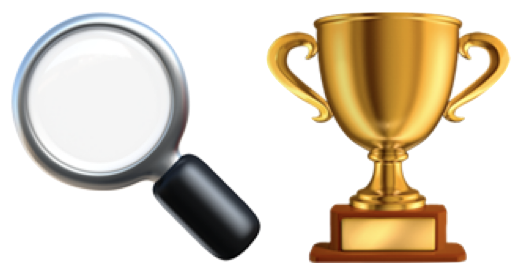
\includegraphics[scale=0.07]{figs/emojis/mini_1.png} & 0 & Target Navigation Effectiveness \\
\hline
\rowcolor{gray!10} 
\includegraphics[scale=0.07]{figs/emojis/mini_2.png} & 0 & Efficient Exploration and Map Memory Utilization \\
\hline
\rowcolor{gray!10} 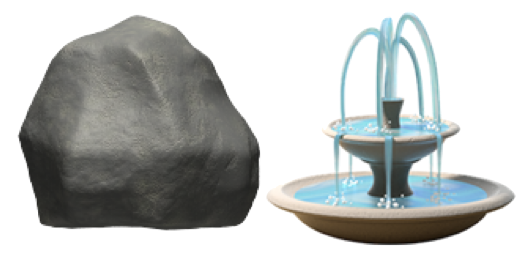
\includegraphics[scale=0.07]{figs/emojis/mini_3.png} & 0 & Hazard Awareness and Equipment Utilization \\
\hline
\rowcolor{gray!10} 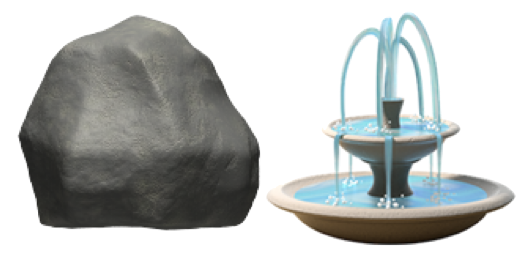
\includegraphics[scale=0.07]{figs/emojis/mini_4.png} & 0 & Boulder Manipulation Strategy \\
\hline
\rowcolor{gray!10} 
\includegraphics[scale=0.07]{figs/emojis/mini_5.png} & 0 & Combat Engagement and Survival \\
\hline
\rowcolor{gray!10} 
\includegraphics[scale=0.07]{figs/emojis/mini_6.png} & 0 & Role-Specific Ability Utilization  \\
\hline
\rowcolor{gray!30} 
\includegraphics[scale=0.07]{figs/emojis/mini_7.png} & 1 & Spatial Awareness and Interpretation  \\
\hline
\rowcolor{gray!30} 
\includegraphics[scale=0.07]{figs/emojis/mini_8.png} & 1 & Object Pickup Efficiency \\
\hline
\rowcolor{gray!60} 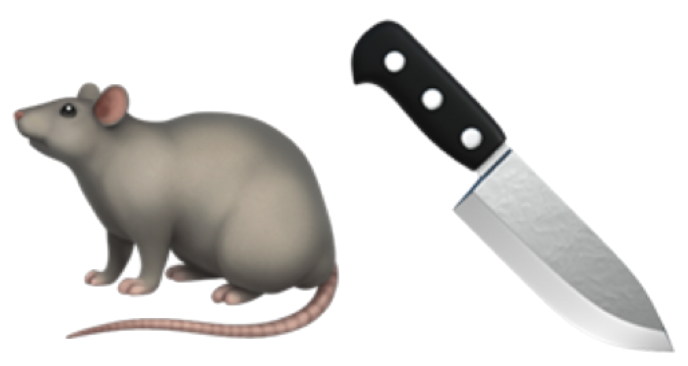
\includegraphics[scale=0.07]{figs/emojis/mini_9.png} & 2 & Giant Rats Encounter Handling \\
\hline
\end{tabular}
\caption{Metrics and Turn of Introduction for MiniHack}
\end{table}

